\chapter[The present AWAKE eBPM system]{The present AWAKE eBPM system}

AWAKE uses a copropagating electron and proton beam. The proton beam has a repetition rate of 10 Hz, while the proton beam from the SPS comes with time intervals in the order of the minute(s).

The simultaneous, shot-by-shot, measurement of the position of the electron and proton beams is desirable. All the experiments so far conduced assuming that the electron position did not drift in the shot with protons. The presence of protons blinds the present electron diagnostic.

\section[Equipment description]{Equipment description}

\subsection[Beamline and diagnostic]{Beamline and diagnostic}

Description of the SPS beamline, of the electron beamline and general other instrumentation installed (including the proton BPMs).

\subsection[Electron BPMs]{Electron BPMs}

The electron beam position monitoring system of the AWAKE facility was developed at TRIUMF\footnote{TRIUMF, Canada's Particle Accelerator Centre, Vancouver, BC, Canada, \url{https://www.triumf.ca/}}. It is composed by shorted stripline-type beam position monitor, and the readout electronics in charge of the signal processing.

\subsubsection{Beam position monitor}

Two types of beam position monitors are installed in the beamlines. In the electron beamline 40 mm aperture BPMs are used, while in the common beamline the 60 mm aperture model is used. The working principle is the same and they differ mostly on the mechanical dimensions. The coverage angle is 38 degrees, with a longitudinal lenght of 120 and 124 mm, respectively.

\subsubsection{Readout electronics}

GENERALITIES ON THE ELECTRONICS


\section[Signal generation]{Signal generation}

The signal is the convolution of the beam spectrum and the pickup response function (is it appropriate to speak of transfer function???). Some words on delta/sigma.

\subsection[Pickup response]{Pickup response}

Lobes and BPM details for shorted striplines

\subsection[Beam spectrum]{Beam spectrum}

In the AWAKE experiment a short electron bunch is propagating in close temporal and spacial proximity with a long proton bunch before entering the plasma cell. The beam parameters are reported in Tab.~\ref{beam_param_exp:tab}. Due to the different bunch length and charge, signals with different bandwidth and magnitude are expected from the two bunches. Figure~\ref{gauss_bunch} shows the time signals and the frequency spectrum of a 250 ps-sigma, 3e11 ppb proton bunch and a 1 ps-sigma, 600 pC electron bunch. From plot (b) it is trivial to see that around $\approx2$~GHz the power of the electron and proton bunch signal has equal strength. At lower frequencies the proton component dominates, while at higher frequencies the electron component has a higher power.

\begin{figure}[ht]
\centering
\subfigure[]
  {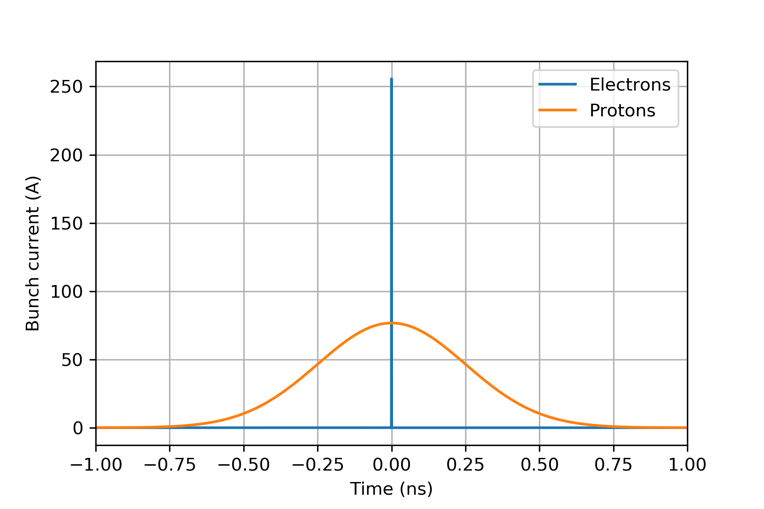
\includegraphics[width=6.5cm,height=5cm]{pictures/gauss_time}}
\hspace{3mm}
\subfigure[]
  {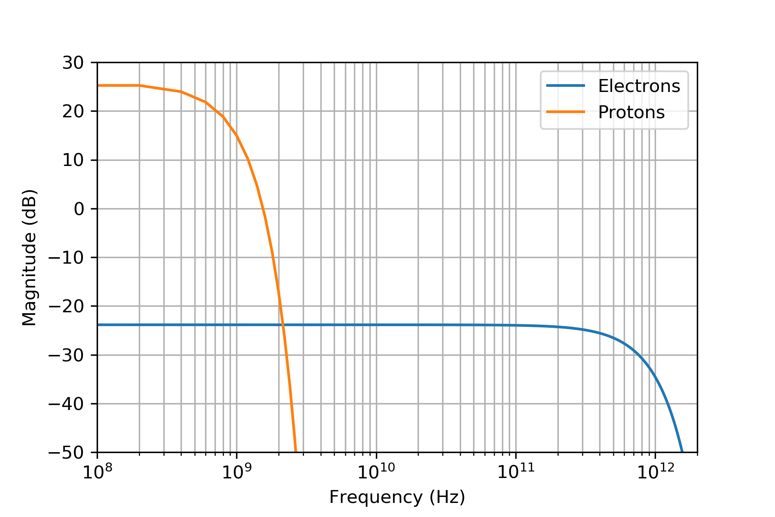
\includegraphics[width=6.5cm,height=5cm]{pictures/gauss_spectrum}}
\caption{The bunch in time (a) and frequency (b) with the paramters of the proton and electron bunch reported in Tab.~\ref{beam_param_exp:tab}.}
\label{gauss_bunch}
\end{figure}

Effect of a non-gaussian proton bunch. Extends more in spectrum.

It is reasonable to assume the electrons as gaussian (QUOTE)




\section[Measurements]{Measurements}

A number of measurements performed on BPM51 with and without beam

\subsection[Electrode signals]{Electrode signals}

with and without proton beam

\subsection[VNA measurements]{VNA measurements}

40 and 60 mm type

\subsubsection[60 mm aperture model]{60 mm aperture model}

60

\subsubsection[40 mm aperture model]{40 mm aperture model}

40



\section[Electromagnetic simulations]{Electromagnetic simulations}

A 3D simplified and parametric model was created in CST STUDIO SUITE\textregistered~2018 on the basis of the drawings provided by TRIUMF that were used for the series production. A new model was created from scratch instead of using the drawings in order to have the full control on the geometrical dimensions and gain in simplicity. This will be exploited when trying to optimise the design, as explained in Section~\ref{sec:optimisations}. A comparison between the two showed that they agree within the mechanical tolerances provided in the design. The the CST model and its comparison to the TRIUMF drawings are shown in Fig.~\ref{STEP_tipp} and Fig.~\ref{CSTvsSTEP_section}. It is important to note that none of the vacuum feedthrough was modeled in CST, as it is inaccurately reported also in the technical drawings as it constitutes industrial secret. In the simulations the signal is collected from the striplines through waveguide ports placed at the end of coaxial lines. The central cilindrical pin of the coaxial line is retained at the design value, while the surrounding vacuum diameter was selected in order to match the line impedance to $50\,\Omega$, in order to avoid unwanted reflections.

The beam position monitor geometry is transversely symmetric. Whenever possible, this has been used to reduce the computing time, imposing boundary conditions.

The simulations regarded mostly calculating the signal response to the beam excitation with different bunch lenghts and the full characterisation of the device as a four port network, calculating the scattering parameters. The former is realised via wakefield simulations, and the latter via frequency domain simulations.

\begin{figure}[ht]
\centering
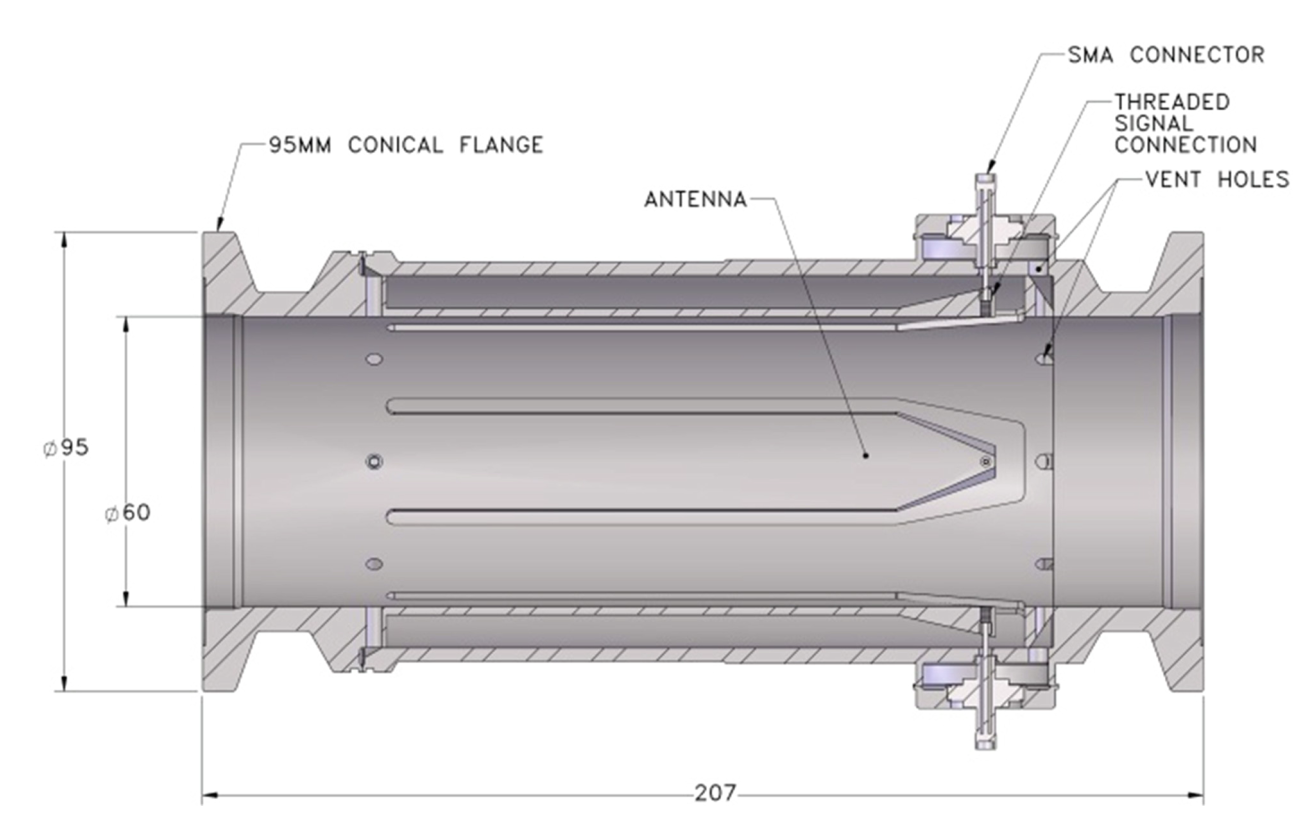
\includegraphics[width=10cm,keepaspectratio]{pictures/tipp_paper}
\caption{Schematic representation of a 60 mm aperture BPM\cite{Shengli:tipp}.}
\label{STEP_tipp}
\end{figure}

\begin{figure}[ht]
\centering
\subfigure[CST model]
  {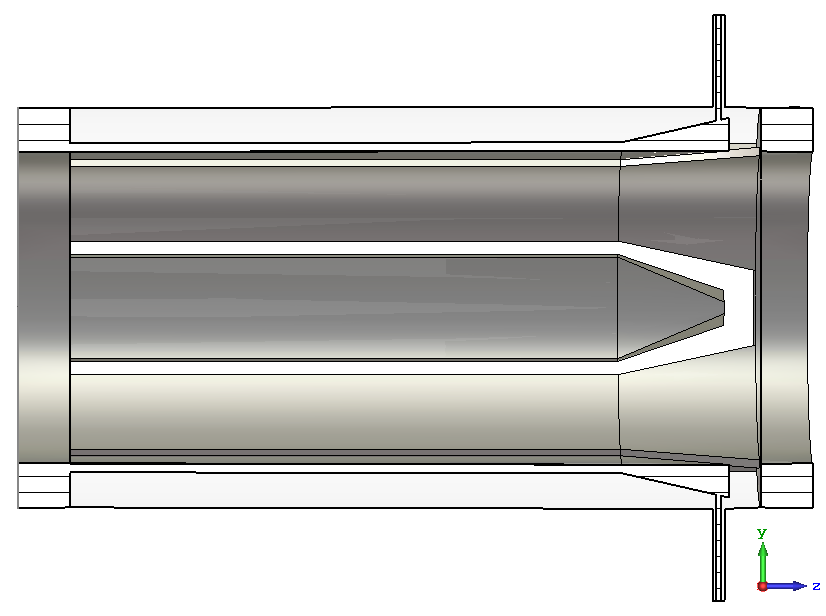
\includegraphics[width=6.5cm,height=5cm]{pictures/CST_section}}
\hspace{3mm}
\subfigure[TRIUMF mechanical model]
  {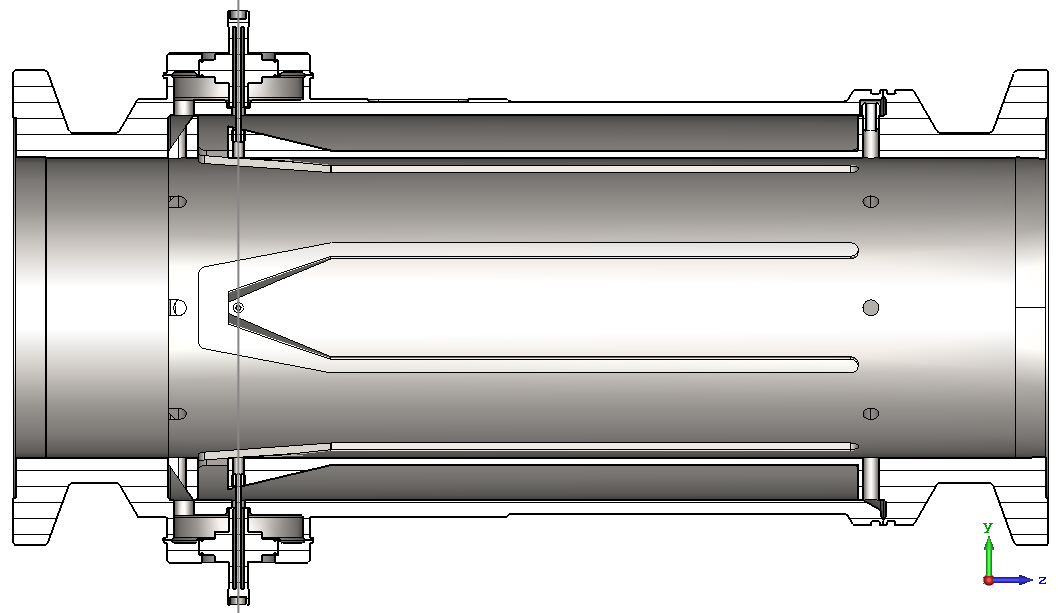
\includegraphics[width=6.5cm,height=5cm]{pictures/STEP_section}}
\caption{3D models used in the electromagnetic simulations (a) and the original mechanical design (b).}
\label{CSTvsSTEP_section}
\end{figure}


\subsection[Electrode signals]{Electrode signals}

Wakefield time domain simulations have been conduced using CST in order to evaluate the stripline response to the beam excitation. This type of simulation assumes a Gaussian beam. The beam parameters were chosen starting from the nominal proton beam used in the experiments, and the charge and bunch length was gradually decreased until reaching the electron beam parameters. Using wakefield simulation it is not possible to simulate both beams travelling in the vacuum pipe together. The simulated beam parameters are reported in Tab.~\ref{beam_param_wak:tab}.

\begin{table}[ht]
  \centering
    \begin{tabular}{l c c c}
    \toprule
    Name  & \multicolumn{2}{c}{Charge} & $\sigma$\\
          & nC & ppb & ps\\
    \midrule
    Proton beam								& $48$	  & $3\times10^{11}$	& 250	\\
    Proton beam/10						& $4.8$	  & $3\times10^{10}$	& 25	\\
    Proton beam/100						& $0.48$  & $3\times10^{9}$		& 2.5	\\
    Electron beam							& $0.6$	  & $3.7\times10^{9}$	& 1		\\
    \bottomrule
    \end{tabular}
  \caption{Beam parameters used in the wakefield simulations} \label{beam_param_wak:tab}
\end{table}




\subsection[Four-port device characterisation in simulations]{Four-port device characterisation in simulations}

Frequency domain simulations were carried out to characterise the BPM as a four port network, in order to compare to the VNA measurements carried out in the laboratory and in the tunnel. For simmetry reasons, it is sufficient to simulate half the structure obtaining anyway the full characterisation of the device including the cross-coupling between the electrodes.





\subsection[Sensitivity studies to the beam position]{Sensitivity studies to the beam position}

Sensitivity study for a proton-like beam


\section[Comparison between measurements and simulations]{Comparison between measurements and simulations}

comp


\section[Design optimisations]{Design optimisations}
\label{sec:optimisations}

\subsection[Impedance matching of the stripline termination]{Impedance matching of the stripline termination}

TDR studies showed that the impendance matching to 50~$\Omega$ of the striplines is not sufficiently optimised. In the attempt of understanding if this could be the source of the resonant response of the device, an geomterical optimisation of the tapered part of the stripline has been carried out. This is realised via parametric time domain simulations, observing the variation of the TDR response. Successively, a wakefield simulation was carried out with the improved geometry, comparing the electrode signal to the unoptimised version.

Something something ...

Mention that in the development phase, this geometry was optimised using the ANSYS\textregistered~HFSS\texttrademark~electromagnetic simulation code\footnote{\url{https://www.ansys.com/products/electronics/ansys-hfss}}, but it had to be modified due to manufacturing constraints during the mechanical design phase\cite{Victor:private-comm}


\subsection[Geometrical optimisation of the space behind the stripline]{Geometrical optimisation of the space behind the stripline}

Same process, but for the



\section[Conclusions]{Conclusions}
